% Drawing 80/01-8 -- folder 80, batch 01, archive page 14 (PDF page 15).
% Transcription: feuille de dessins au stylo et au crayon : à gauche cinq droites $D_0$ (horizontale, épaissie), $D_1$, $D_2$, $D_3$, $D_4$ formant une étoile à cinq branches, les deux triangles inférieurs hachurés, de longs traits parallèles au crayon descendant sous l'étoile ; à droite de $D_0$, un « $D_0'$ » raturé ; plus à droite une courbe (pseudo-droite) descendant du haut vers le bas à droite ; à droite encore, quatre petits croquis de deux ou trois droites sécantes, un côté de chaque droite marqué de hachures
% Kind: pentagram of five lines D_0..D_4 with hatched triangles, a curve and four small sketches. Method 2 (schematic redraw from the facsimile). Status: partial.
% Notes: The five lines are drawn through the ten crossing points of the star, each point shared. D_0 heavy between D_1 and D_4 and beyond; D_2 bends down at its lower right end and D_3 is bent, as on the page. Hatching of the two lower triangles and of the tip above the top crossing is schematic (a few strokes each); five long pencil strokes below the star stand for the parallel strokes of the page. The curve on the right and the four small sketches (lines with hatching on one side) are redrawn stroke by stroke, their hatching schematic. Left out: the struck label D_0' at the right end of D_0 (strike-outs are not drawn) and faint pencil traces at the bottom of the sheet. Redrawn 2026-11-12 (issue 128): to check again. 2026-11-14, Claude Opus 5.5, overlay check (issue 147): rasterised from its own coordinates over the 400 dpi colour scan on a unit grid and measured; not compiled (no TeX in the session). The five lines D_0 to D_4 with their crossings, the bend of D_2 and D_3, the labels, the curve on the right and the main strokes of the four small sketches lie on their ink to within about 1 unit. Changed: the hatching of the two lower triangles is now the page's strokes, read one by one (five in each, nearly vertical, falling from the upper side; the earlier schematic strokes fell the other way and crossed them); two of the long pencil strokes below the star moved onto their pencil. Still differs, and why it stays partial: the hatching of the tip above the star and of the four small sketches is still a few evenly spaced strokes, not his (their strokes are short and overlap the lines they hatch); the long pencil strokes below the star are at the limit of what the scan shows (the faintest is not picked up by a measure of the ink at all), so their number and ends remain a reading.
% Coordinates: 1 unit = 1 mm = 1/100 of the crop width (bbox in page fractions: [0.1, 0.07, 0.99, 0.515]).
% Redrawn by Claude (claude-fable-5-2), issue #128, 2026-11-12; not checked by a human; not compiled (no TeX in the session).
% Checked by Claude (claude-opus-5-5) 2026-11-14 (issue #147): overlaid on the 400 dpi colour facsimile, corrected; not compiled (no TeX in the session). Not checked by a human. Status: partial.
% Rights: reproduces part of the work -- behind RENDER_TRANSCRIPTS, never published by itself.
\documentclass[tikz,border=3pt]{standalone}
\usepackage{amsmath,amssymb}
\usetikzlibrary{patterns,arrows.meta}
\tikzset{pencil/.style={black!45}, struck/.style={black!35}, mpt/.style={circle,draw,inner sep=1.3pt}, pt/.style={circle,fill,inner sep=0.9pt}, opt/.style={circle,draw,fill=white,inner sep=1.1pt}}
\begin{document}
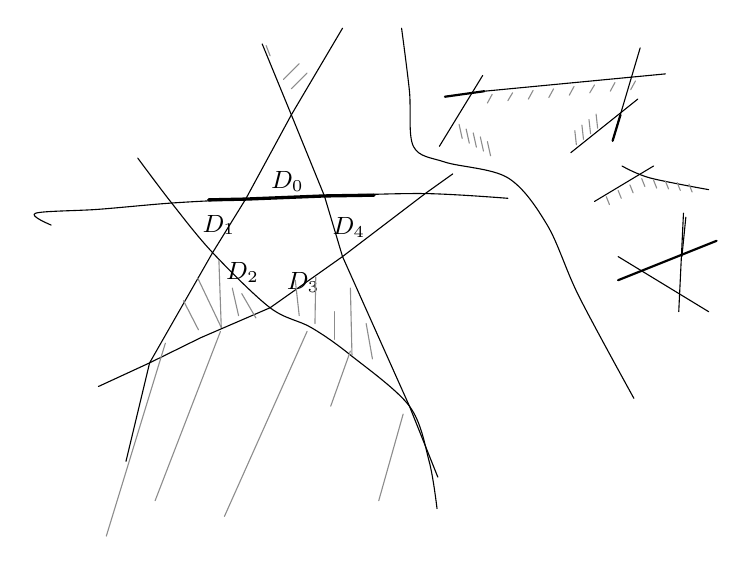
\begin{tikzpicture}[x=1mm,y=1mm,line cap=round,line join=round,font=\scriptsize]
\draw plot[smooth, tension=0.55] coordinates {(14,-27) (12,-25.5) (20,-25) (29.3,-24.2) (38.7,-23.7) (48.7,-23.3) (61.5,-23) (72,-23.6)};
\draw[very thick] (34,-23.8) -- (38.7,-23.7) -- (48.7,-23.3) -- (55,-23.2);
\draw (51,-2) -- (44.5,-13) -- (38.7,-23.7) -- (34.5,-30.5) -- (26.5,-44.5) -- (23.5,-57);
\draw (40.8,-4) -- (44.5,-13) -- (48.7,-23.3) -- (51,-31) -- (59.5,-50) -- (63.1,-59);
\draw plot[smooth, tension=0.55] coordinates {(25,-18.5) (29.3,-24.2) (34.5,-30.5) (41.8,-37.5) (47,-40) (52,-43.5) (59.5,-50) (62,-57) (63,-63)};
\draw (20,-47.5) -- (26.5,-44.5) -- (33,-41.3) -- (41.8,-37.5) -- (51,-31) -- (61.5,-23) -- (65,-20.5);
\node[inner sep=1pt] at (44,-21.5) {\small $D_0$};
\node[inner sep=1pt] at (35.3,-27) {\small $D_1$};
\node[inner sep=1pt] at (51.8,-27.3) {\small $D_4$};
\node[inner sep=1pt] at (38.3,-33) {\small $D_2$};
\node[inner sep=1pt] at (46,-34.3) {\small $D_3$};
\draw[pencil] (43.5,-8.5) -- (45.5,-6.5);
\draw[pencil] (44.5,-9.7) -- (46.5,-7.7);
\draw[pencil] (41.3,-4.2) -- (41.8,-5.5);
\draw[pencil] (30.8,-36.6) -- (32.7,-40.3);
\draw[pencil] (32.6,-33.7) -- (35.6,-40);
\draw[pencil] (35.3,-31.5) -- (35.6,-40);
\draw[pencil] (37,-35) -- (37.8,-38.5);
\draw[pencil] (38.2,-35.7) -- (40,-38.8);
\draw[pencil] (45,-34) -- (45.5,-38.5);
\draw[pencil] (47.6,-33.6) -- (47.5,-39.5);
\draw[pencil] (50,-38) -- (50,-41.5);
\draw[pencil] (52,-35) -- (52.2,-43.5);
\draw[pencil] (54,-39.5) -- (54.8,-44);
\draw[pencil] (28.5,-42) -- (21,-66.5);
\draw[pencil] (35.5,-40.5) -- (27.2,-62);
\draw[pencil] (46.5,-40.5) -- (36,-64);
\draw[pencil] (52,-43) -- (49.5,-50);
\draw[pencil] (58.7,-51) -- (55.6,-62);
\draw plot[smooth, tension=0.55] coordinates {(58.5,-2) (59.5,-10) (60,-17) (64,-19) (72,-21) (77,-27) (81,-36) (88,-49)};
\draw[thick] (64,-10.7) -- (69,-10);
\draw (69,-10) -- (92,-7.8);
\draw (68.8,-8) -- (63.3,-17);
\draw[pencil] (70,-10.4) -- (69.4,-11.5);
\draw[pencil] (72.6,-10.2) -- (72,-11.2);
\draw[pencil] (75.2,-9.9) -- (74.6,-11);
\draw[pencil] (77.8,-9.7) -- (77.2,-10.8);
\draw[pencil] (80.4,-9.4) -- (79.8,-10.5);
\draw[pencil] (83,-9.2) -- (82.4,-10.2);
\draw[pencil] (85.6,-8.9) -- (85,-10);
\draw[pencil] (88.2,-8.7) -- (87.6,-9.8);
\draw[pencil] (65.8,-14.2) -- (66.2,-16);
\draw[pencil] (66.7,-14.8) -- (67.1,-16.6);
\draw[pencil] (67.6,-15.3) -- (68,-17.1);
\draw[pencil] (68.5,-15.8) -- (68.9,-17.6);
\draw[pencil] (69.4,-16.4) -- (69.8,-18.2);
\draw (80,-17.8) -- (88.5,-11);
\draw (88.8,-4.5) -- (85.3,-16.3);
\draw[thick] (86.3,-13) -- (85.3,-16.3);
\draw[pencil] (80.7,-16.8) -- (80.5,-15);
\draw[pencil] (81.6,-16.1) -- (81.4,-14.3);
\draw[pencil] (82.5,-15.4) -- (82.3,-13.6);
\draw[pencil] (83.4,-14.7) -- (83.2,-12.9);
\draw (83,-24) -- (90.5,-19.5);
\draw plot[smooth, tension=0.55] coordinates {(86.5,-19.5) (90,-21) (97.5,-22.5)};
\draw[pencil] (84.5,-23.4) -- (84.9,-24.4);
\draw[pencil] (86,-22.6) -- (86.4,-23.6);
\draw[pencil] (87.5,-21.9) -- (87.9,-22.9);
\draw[pencil] (89,-21.1) -- (89.4,-22.1);
\draw[pencil] (90.5,-21.3) -- (90.9,-22.3);
\draw[pencil] (92,-21.4) -- (92.4,-22.4);
\draw[pencil] (93.5,-21.6) -- (93.9,-22.6);
\draw[pencil] (95,-21.8) -- (95.4,-22.8);
\draw (94.3,-25.5) -- (93.7,-38);
\draw (94.6,-26) -- (94.1,-31);
\draw[thick] (86,-34) -- (98.5,-29);
\draw (86,-31) -- (97.5,-38);
\end{tikzpicture}
\end{document}
